\chapter{Low Energy Electron Diffraction LEED}
\section{Surface Crystallography}
Surface crystallography is just a special case of bulk crystallography where the crystal has been divided by a mathematical plane. We will only consider the terminology involving surfaces and some of the most often used concepts and encountered structures for metals namely Face Centered Cubic (FCC) Body Centered Cubic (BCC) and Hexagonal Close-Packed (HCP) lattices shown in \autoref{fig:unitcells}. For the more special structures like for instance the diamond structure we will refer to the literature \cite{Kittel, Ashcroft}.

\begin{figure}[h!]
	\begin{center}
	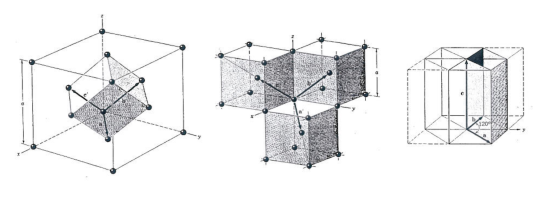
\includegraphics[scale=4]{figures/09_01.png}
	\caption{The unit cell for the FCC, BCC, and HPC lattices.}
	\label{fig:unitcells}
	\end{center}
\end{figure}

\subsection{Crystal Planes}
Since the surface structure and geometry is very important in many cases, for example when considering reactivity, and since it differs a lot from one surface structure to another it is important to have a notation that describes the various surfaces in a unique manner. The crystal surfaces are described by the vector normal to the surface given by

\begin{equation}
\vec{H}=h\vec{x}+k\vec{y}+l\vec{z}
\end{equation}

\noindent and the  notation is the name of the substrate and the surface normal vector $(hkl)$, for example Cu(100). Please note that the permutations Cu(100), Cu(010), and Cu(001) all describes the same surface as shown in \autoref{fig:basalplanes} for the cubic crystals. Negative numbers are noted by a bar over the number so Cu(100) is naturally equal Cu(0$\overline{1}$0). The three basal planes for the cubic crystals are (100), (110) and the (111). The respective cuts are shown in \autoref{fig:basalplanes} and the relative positions of the surface atoms are shown in \autoref{fig:surfaces}.

\begin{figure}[h!]
	\begin{center}
	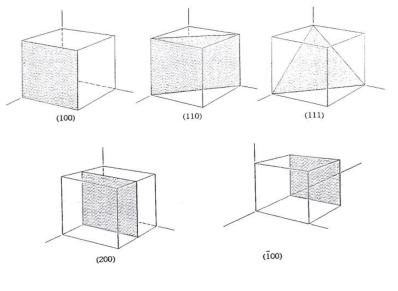
\includegraphics[scale=4]{figures/09_02.png}
	\caption{The basal planes formed by cuts of the unit cells of the simple crystal structures.}
	\label{fig:basalplanes}
	\end{center}
\end{figure}

An important parameter for surfaces are often the density of atoms in the surface. Note that for FCC crystals the (110) is the most open whereas the (111) is the most close packed. For BCC crystals it is the opposite order i.e. the (111) most open and (110) most close packed. Also more complicated surface structures containing steps or even kinks may be described in this notation as $n(h_tk_tl_t)\times(h_sk_sl_s)$ where $n$ describes that the surface contains $n$ rows of atoms forming a terrace of $(h_tk_tl_t)$ and one step of type $(h_sk_sl_s)$. Thus a (775) surface is equivalent to $6(111)\times(11\overline{1})$. In this manner all sorts of surfaces may be constructed, but the question is naturally whether they are stable or will facet into other structures.

\begin{figure}[h!]
	\begin{center}
	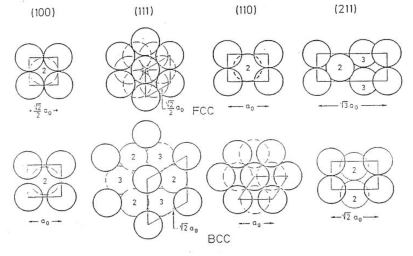
\includegraphics[scale=4]{figures/09_03.png}
	\caption{The surface structures of the basal planes for the FCC and BCC.}
	\label{fig:surfaces}
	\end{center}
\end{figure}

A particular surface structure may be prepared by spark cutting a single crystal normal to the desired direction. The crystal is usually oriented by Laue X-ray diffraction with an accuracy better than \ang{0.5}. The surface is then polished with polish paste with decreasing grain size until all scratches etc. are removed and a mirror like surface is obtained. Sometimes, in particular for the soft materials like Cu, an additional electro polish is needed to remove damaged layers. Finally the crystal is mounted in the UHV chamber and is cleaned by repeated cycles of sputtering and annealing. Getting a clean single crystal surface may be tedious work and may take several months. The cleaning procedure varies from element to element and usually effective and successful recipes can be found in the literature.

\subsection{Adsorbate Sites}
The definition of the most frequent  adsorption sites are shown in \autoref{fig:adsorptionsites}. They are named on-top site, bridge sites  (may be long or short bridged), and hollow sites which may be three fold hollow or four fold hollow. In for example the FCC(111) cases it is also necessary to distinguish between HCP and FCC sites describing whether there is an atom just below the site or it is in the second layer.

\begin{figure}[h!]
	\begin{center}
	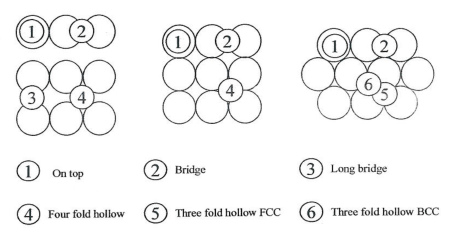
\includegraphics[scale=3.5]{figures/09_04.png}
	\caption{The adsorption sites for various surface geometries.}
	\label{fig:adsorptionsites}
	\end{center}
\end{figure}

\subsection{The Two-Dimensional Lattice}
A two-dimensional structure processing periodicity can be described by a two dimensional lattice. Any point in this lattice can be reached by a suitable combination of basis vectors. Two unit vectors will describe the smallest cell in which an identical arrangement of the atoms is found. The whole lattice can then be described by moving this unit cell by any linear combination of the unit vectors. These vectors form the {\it Bravais} lattice which is the set of vectors by which all points in the lattice can be reached.

\section{Low Electron Energy Diffraction}
\subsection{Experimental Set-up}
Having defined the fundamental structure we will now turn to the Low Electron Energy Diffraction Experiment (LEED). The first experiment made realising that electrons could be used for investigating surface structures was made by Davidson and Germer in 1927 \cite{Davidson}, but as the crystals could not be kept clean (due to poor vacuum) it was not until the late sixties that the method started to take off. Several excellent reviews and monographs have been written on this subject \cite{Pendry, Hove, Heinz, Ertl}. The experiment relies on the duality of electrons which in some case should be considered as particles and under other conditions as wave packets. If we choose to use electrons with energy around the minimum in the universal curve (Fig. \ref{fig:mean_free_path}) (\SIrange{40}{200}{\electronvolt}) where we have the maximum surface sensitivity the wavelength of the electrons will be comparable with the lattice distance of single crystals considered here.

\begin{eqnarray}
\lambda	& =	& \frac{h}{p}\\
p	& =	& \hbar k=\sqrt{2mE_p}\\
\lambda(\si{\angstrom})	& =	& \sqrt{\frac{150.4}{E_p(\si{eV})}}
\end{eqnarray}

This means that the electrons may be scattered elastically  in the surface and undergo constructive and destructive interference. The back scattered electrons are then analysed and from that the symmetry of the surface may be deduced.

The experimental set-up is shown in \autoref{fig:leed}.  A beam of electrons with energy $E_p$ from a relative simple electron gun mounted in the center of the LEED optics is directed towards the surface. The crystal is mounted so it can be positioned in the center of three concentric hemispherical grids. The inner grid is grounded whereas the middle grid is kept on a negative potential slightly below $E_p$ so only electrons which have not undergone any energy losses are allowed to pass. Between the last grid and an outer fluorescent screen there are a potential difference between \SIrange{2}{5}{kV} so the electrons that pass are accelerated towards the fluorescent screen where they will form observable spots. The screen is  transparent so the spots can be observed from behind it as well without being obstructed by the sample mount. The spots can then be photographed or followed by a CCD camera. More elaborate set-ups have been constructed for Spot Profile Analysis LEED (SPALEED) where the detailed profile can reveal details on the long range structure, but that will not be considered here.

\begin{figure}[h!]
	\begin{center}
	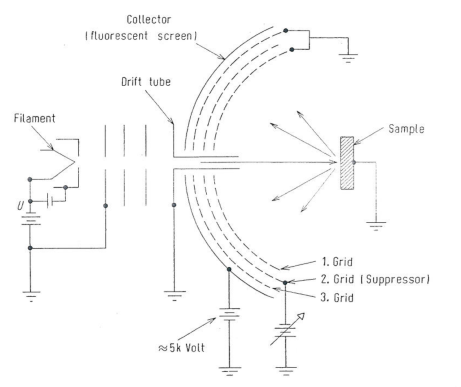
\includegraphics[scale=4]{figures/09_05.png}
	\caption{Schematic drawing of LEED optics.}
	\label{fig:leed}
	\end{center}
\end{figure}

\begin{figure}[h!]
	\begin{center}
	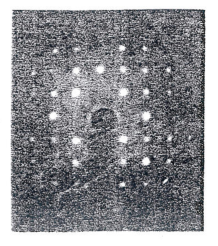
\includegraphics[scale=4]{figures/09_06.png}
	\caption{LEED pattern obtained from a Cu(100) surface reconstructed by adsorption of atomic hydrogen. The energy of the electrons was relatively high $E_p=\SI{178}{\electronvolt}$ and the beam was  normal to the surface. Only the bright spots are observed on a clean Cu(100). From \cite{HonCu}.}
	\label{fig:culeed}
	\end{center}
\end{figure}

Such a LEED pattern is reproduced in \autoref{fig:culeed} \cite{HonCu}.

The principle of the experiment is shown schematically in \autoref{fig:leedsketch} where an incoming electron beam interacts with a crystal described by $\vec{a_1}$ and $\vec{a_2}$. The (00) beam is reflected directly back into the electron gun and can therefore not be observed unless  the crystal is tilted.

The intensity of the spots formed on the screen can also be followed as a function of primary energy $E_p$. The spots will move towards the zero order spot with increasing energy and then varying strongly in intensity. The diffraction in the two-dimensional lattice lead to the diffracted beams indicated in \autoref{fig:leedsketch} whereas the $d$ modulation of the intensity as a function of $E_p$ is due to diffraction between subsequent layers into the crystal. We will first concentrate on understanding the diffraction pattern which reveals the two-dimensional symmetry of the surface layers and in the end of this chapter  briefly touch upon the intensity variation, which can be used to determine the distances in the surface structure.

\begin{figure}[h!]
	\begin{center}
	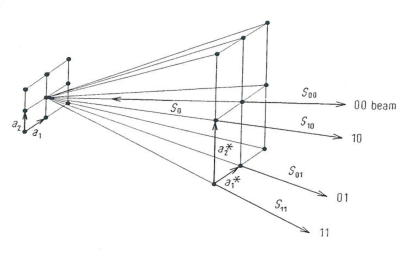
\includegraphics[scale=4]{figures/09_07.png}
	\caption{Sketch of the LEED experiment on a single crystal spanned by $\vec{a_1}$ and $\vec{a_2}$.}
	\label{fig:leedsketch}
	\end{center}
\end{figure}

\subsection{Kinematic Theory}
The direction of the diffraction beams can be found by first considering what happens when an electron interacts with  atoms in the surface. The differential scattering cross section for an elastic collision of an electron with a fixed atom is given by the asymptotic solution to the Schr\"{o}dinger equation:

\begin{equation}
\frac{-\hbar^2}{2m}\nabla^2\Psi +V\Psi =E\Psi
\end{equation}

Far away from the atom $V=0$ and the asymptotic solution to $\Psi$ can be written as a sum of an incoming plane wave and an outgoing spherical wave:

\begin{equation}
\Psi =e^{i\vec{k}\vec{r}}+f(\alpha,\phi)\frac{e^{i\vec{k}\vec{r}}}{\vec{r}}
\end{equation}

\noindent where $f(\alpha,\phi)$ is the amplitude of the outgoing electron and $\vert f(\alpha,\phi)\vert^2$ is the differential scattering cross section which must be found by solving the Schr\"{o}dinger equation in the vicinity of the atom where $V\neq 0$. $\alpha$ and $\phi$ are the angles of the scattering. Assuming that the potential is spherically symmetrical the solutions to the Schr\"{o}dinger equations are separable in the coordinates $r, \alpha, \phi$ and the wave functions are of the hydrogen type namely a product of radial and spherical harmonic:

\begin{equation}
\Psi_n(r,\alpha,\phi)=R_n(r)\Upsilon_{l,m}(\alpha,\phi) 
\end{equation}

\noindent where $n, l$ and $m$ are the principal, azimuthal and magnetic quantum numbers, respectively.

The amplitude of the scattered electrons can  be described as an expansion of phase shifted Legendre polynomials where the phase shift comes from the interaction with the potential $V$. Usually a band structure potential have been used for $V$ when describing atoms in a solid. For details on scattering of electrons on potentials we will refer to standard quantum mechanics \cite{Shiff,Merzbacher}.

What happens when considering more than one  atom scattering the incoming electrons? Firstly, consider a plane wave scattering on two atoms separated by a distance of $R$. This would lead to two spherical waves interfering at the position of the observer (see Fig. \ref{fig:electronscatter}). The difference in phase of the two waves $\Delta$ is given by

\begin{figure}[h!]
	\begin{center}
	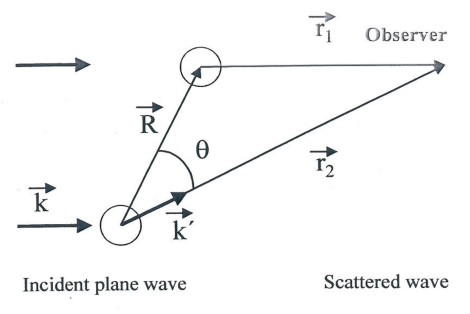
\includegraphics[scale=2]{figures/09_08.png}
	\caption{An incoming electron with wave vector $\vec{k}$ scatters on two atoms with distance $\vec{R}$.}
	\label{fig:electronscatter}
	\end{center}
\end{figure}

\begin{equation}
\Delta=e^{i\vec{k} \vec{R}+i\vec{k} \vec{r_1}-i\vec{k'}\vec{r_2}} 
\end{equation}

If the observer is far away, which is always the case here, then $\vec{r_1}\approx\vec{r_2}\gg \vec{R}$ leading to $r_2\approx r_1+R\cos(\theta)$, thus

\begin{eqnarray}
\Delta	& =		& e^{i\vec{k}\vec{R}+ik_xr_1-ik'_x(r_1+R\cos\theta)+ik'_yR\sin\theta)}\\ 
\Delta	& \approx	& e^{i\vec{k}\vec{R}-ik'_x(R\cos\theta)+ik'_yR\sin\theta} \mbox{, Since } k_x\approx k'_x\\
\Delta	& \approx	& e^{i\vec{k}\vec{R}-i\vec{k'}\vec{R}}=e^{i(\vec{k}-\vec{k'})\vec{R}}=e^{i\vec{\Delta k}\vec{R}}
\end{eqnarray}

\noindent where $\vec{k^\prime}$ is parallel to $\vec{r_2}$ and  $\vec{\Delta k}$ is the difference between $\vec{k}$ and $\vec{k^\prime}$.

The amplitude of the wave seen by the observer will be  proportional to the phase difference. If we now turn to a unit cell which may contain several different atoms the amplitude from this  $F(\Delta k)$ can be found by summing over the contributions from the $i$'th atom in the unit cell as

\begin{equation}
F(\vec{\Delta k})=\sum_i f_i(\vec{\Delta k})e^{i\vec{r_i}\vec{\Delta k}}
\end{equation}

\noindent where $f_i$ is the so called "form factor" which is dependent on the potential for the various atoms.

Let us now consider a two-dimensional lattice described by the vectors $\vec{a_1}$ and $\vec{a_2}$ as shown in \autoref{fig:leedsketch}. The crystal is considered to be finite and consisting of $M$ atoms in the $\vec{a_1}$ direction and $N$ in the $\vec{a_2}$ direction.

The amplitude $\Delta(\vec{\Delta k})$ from this plane can be found by summing over all the phase differences between the electrons scattered on each unit cell leading to:

\begin{equation}
\Delta(\vec{\Delta k})=F(\vec{\Delta k})\sum_{m=0}^{M-1}e^{im\vec{a_1}\vec{\Delta k}}\sum_{n=0}^{N-1}e^{in\vec{a_2}\vec{\Delta k}}
\end{equation}

Remembering that

\begin{equation}
\sum_{m=0}^{M-1}x^m=\frac{1-x^M}{1-x}
\end{equation}

\begin{equation}
\Delta(\vec{\Delta k})=F(\vec{\Delta k})\frac{(1-e^{iM\vec{a_1}\vec{\Delta k}})(1-e^{iN\vec{a_2}\vec{\Delta k}})}{(1-e^{i\vec{a_1}\vec{\Delta k}})(1-e^{i\vec{a_2}\vec{\Delta k}})}
\end{equation}

It is not the amplitude but the intensity which is interesting so we would have to multiply the amplitude by its complex conjugate and by using the cosine relations we find

\begin{equation}
I(\Delta \vec{k}) = \frac{\sin^2\left(\frac{M}{2}\vec{a}_1 \Delta k_{\parallel}\right) \sin^2\left(\frac{N}{2}\vec{a}_2 \Delta k_{\parallel}\right)}{\sin^2\left(\frac{1}{2}\vec{a}_1 \Delta k_{\parallel}\right) \sin^2\left(\frac{1}{2}\vec{a}_2 \Delta k_{\parallel}\right)}
\end{equation}

\noindent since $\vec{a_1}\vec{\Delta k}=\vec{a_1}\vec{\Delta k_{\parallel}}$ as $\vec{a_1}$ is located in the surface plane.

Now it is possible to see that there will only be an intensity in specific directions namely when the denominator goes towards zero i.e. when:

\begin{eqnarray}
\vec{a_1}\vec{\Delta k_{\parallel}}	& =	& h2\pi \\
\vec{a_2}\vec{\Delta k_{\parallel}} & =	& l2\pi \\
h,l	& \in	& Z
\end{eqnarray}

Thus for a plane of sufficient dimensions and when the observer is far away from the plane the spherical waves scattered from each unit cell will give rise to localised beams diffracted in directions parallel to the surface so they obey the above relations characterised by the indices $h$ and $l$.

\subsubsection{The Reciprocal Lattice}
When having a real-space lattice defined as above where for example

\begin{equation}
\vec{r_{m,n}}=m\vec{a_1}+n\vec{a_2}
\end{equation}

\noindent it is possible to define a reciprocal lattice vector in the plane given by

\begin{equation}
\vec{g_{h,l}}\equiv h\vec{a_1^*}+l\vec{a_2^*}
\end{equation}

\noindent where the basis vectors of the reciprocal lattice are defined as:

\begin{eqnarray}
\vec{a_1^*}	& \equiv	& 2\pi\frac{\vec{a_2}\times\vec{z}}{\vec{a_1}\cdot\vec{a_2}\times\vec{z}}\\
\vec{a_2^*}	& \equiv	& 2\pi\frac{\vec{z}\times\vec{a_1}}{\vec{a_1}\cdot\vec{a_2}\times\vec{z}}
\end{eqnarray}

\noindent where $\vec{z}$ is the vector normal to the surface and the denominator is the volume of the unit cell. 

\begin{equation}
\vec{\Delta k_{\parallel}}=\vec{g_{h,l}}
\end{equation}

This means the diffracted beam occurs when the change in momentum parallel to the surface equals a reciprocal vector or linear combination thereof. Let us try to relate this information to the spot we see on our screen. That we have a spot means that a diffracted beam $(h,l)$ crosses our LEED optics as shown in \autoref{fig:leedcs}. In a conventional LEED optic the radius of the screen $R$ is known. By observing the position of the spot we can thus determine the angle $\theta_{h,l}$ the diffracted beam has been scattered.

\begin{figure}[h!]
	\begin{center}
	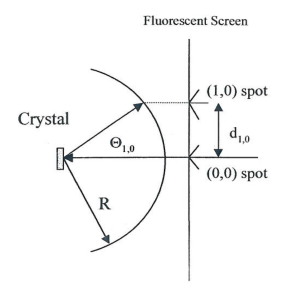
\includegraphics[scale=4]{figures/09_09.png}
	\caption{Cross section of the experimental set-up. Radius of the screen is $R$ and the beam $(h,l)$ gives a spot a distance $d_{h,l}$ measured from the zeroth order spot.}
	\label{fig:leedcs}
	\end{center}
\end{figure}

\begin{equation}
\sin{\theta_{h,l}} = \frac{d_{h,l}}{R} = \frac{g_{h,l}}{k}
\end{equation}

\noindent where $k$ is the wave vector of the electron. (We are assuming normal incidence of the incoming beam. This is not a necessity, but simplifies the experiment). It is seen that the distance seen on the screen $d_{h,l}$ is inversely proportional to the  square root of the energy, meaning that all spots will converge towards the zeroth order spot for high energies as mentioned earlier. This is a good method for identifying  the zeroth order spot. It is also possible to give an estimate of the lattice distance of the crystal by measuring the distance $d_{1,0}$, which is between the first order spot $(1,0)$ and the zeroth order spot $(0,0)$. Since $g_{1,0}=2\pi/a_1$ the lattice distance is given by:

\begin{equation}
a_1=\frac{2\pi R\hbar}{d_{1,0}\sqrt{2mE_p}}
\end{equation}

Since the spots are usually not extremely sharp this is not a very accurate method for determining lattice distances.

\subsubsection{The Coherence Length}
The diameter of the spot seen on the screen depends critically on the level of order on the surface, the quality of the electron beam used and the temperature of the crystal. Let us first assume that we have an ideal electron beam i.e. the electron trajectories are all parallel and the beam is monochromatised. If we look at a spot profile the intensity will be given by:

\begin{equation}
I\left(\vec{\Delta k}\right)=\frac{\sin^2\left(M/2 \vec{a_1}\vec{\Delta k_{\parallel}}\right)}{\sin^2\left(1/2\vec{a_1}\vec{\Delta k_{\parallel}}\right)}
\end{equation}

\noindent which can be approximated as

\begin{equation}
I(x)\propto\frac{\sin^2(x)}{x^2}
\end{equation}

\noindent where $x=M/2\vec{a_1}\vec{\Delta k_{\parallel}}$ and the intensity profile is shown in \autoref{fig:spotprofileint}.

\begin{figure}[h!]
	\begin{center}
	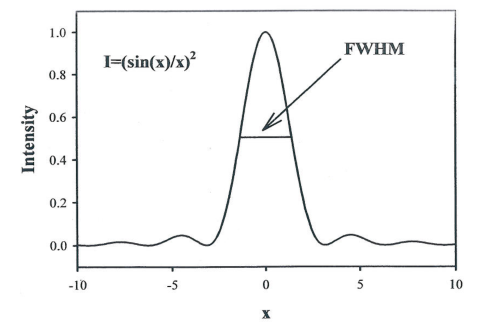
\includegraphics[scale=3]{figures/09_10.png}
	\caption{The intensity of the spot profile as a function of $x$ as defined in the text.}
	\label{fig:spotprofileint}
	\end{center}
\end{figure}

It can be shown that the FWHM of the spot is given by $\vec{a_1}\vec{\Delta k_{\parallel}}=0.44\pi /M$ meaning that if there are just ordered areas bigger than, say, 30 by 30 atoms this effect will no longer contribute significantly  to the  broadening of the observed spots. Thus LEED is not very useful for determining the over all order of a surface since it only reflects the areas that are ordered and discriminates those which are disordered. If one however observes a LEED pattern with diffuse spots the surface order is certainly of poor quality.

Usually it is the quality of the electron gun that sets the limit of how sharp the spots can be. The beam diameter will normally be of the order of \SIrange{0.1}{1.0}{mm}, which is the area the LEED experiment is probing. Unfortunately the beam energy is not monochromatised and completely parallel. The energy resolution is as we shall see of less importance, but both effects contributes to an uncertainty of the parallel momentum $\Delta \Delta k_{\parallel}$  of the incoming beam, which will be reflected in the outgoing beams. This uncertainty in the beam can be translated into a transfer width $W$ given by

\begin{equation}
W=\frac{2\pi}{\Delta \Delta k_{\parallel}}
\end{equation}
 
\noindent where

\begin{equation}
\Delta k_{\parallel}=2\pi\sqrt{\frac{E_p}{150.4}}(\sin(\theta_{out})-\sin(\theta_{in}))
\end{equation} 

By neglecting contributions from $\theta_{out}$ and assuming normal incidence we find the respective uncertainties for divergence and energy by differentiation. From those we can estimate the respective transfer widths to:

\begin{equation}
W_{\theta_{in}}=\frac{\lambda}{\cos(\theta_{in})\Delta\theta_{in}}
\end{equation}

\noindent and 

\begin{equation}
W_{E_p}=\frac{4\pi E_p}{\Delta k_{\parallel}\Delta E_p}
\end{equation}

Substituting realistic values for a conventional LEED system like $E_p=\SI{100}{\electronvolt}$, $\Delta E_p=\SI{0.5}{\electronvolt}$, $\Delta\theta_{in}=\ang{0.6}$ and $2\pi /\Delta k_{\parallel}=\SI{2.5}{\angstrom}$ we get $W_{\theta}=\SI{100}{\angstrom}$ and $W_E=\SI{1000}{\angstrom}$. It is obvious that the uncertainty of the beam convergence is dominating meaning that as long as we have ordered islands on the surface that are larger than the transfer width of our LEED optics we will not be able to notice an effect on the sharpness of the spots. Normally we are talking about a coherence length on the order of \SIrange{100}{200}{\angstrom} meaning that we can have a crystal which in LEED will appear well ordered, but locally may have areas that are completely disordered. This may first be realised when Scanning Tunneling Microscopy (STM) experiments are performed since that method is very sensitive to the local order. By optimising the experimental set-up it is possible to obtain electron beams in which the electron trajectories are parallel to a high degree. In this manner the uncertainty of the angle can be eliminated and long range order may be observed. The detail are investigated by spot profile analysis and referred to as SPALEED. The experiment requires dedicated equipment and is commercially available.

For completeness it should also be mentioned that the temperature of the sample have a profound effect on the spot profile since the atoms in the surface oscillates due to the phonons. This gives an uncertainty of the positions of the surface atoms which will naturally result in a decreasing intensity and broadening of the LEED spots. Thus it is preferable to stay at room temperature or lower when doing LEED experiments.The intensity is given by:

\begin{equation}
I=I_0e^{-2M}
\end{equation}

\noindent where

\begin{equation}
2M=\frac{12h^2T}{mk_B\theta_D^2}\left(\frac{\cos(\phi)}{\lambda}\right)^2
\end{equation}

\noindent where $\phi$ is the scattering angle, $\lambda$ is the wavelength, and $\theta_D$ is the Debye temperature. By plotting $\log{I}$ vs. temperature the Debye temperature can be extracted. At low mean free paths it will primarily be the Debye temperature of the surface layer which is lower than that of the bulk.

\subsection{Multiple Scattering}
Above we have only considered one plane of atoms but the scattering process will in general always take place in several non-equivalent layers. This is the effect that will cause modulation of the diffracted beam as mentioned earlier leading to the IV-curves. A first glance one could expect the resulting LEED patterns just to be a sum of the scattering in the different non-equivalent planes. This would be the case if the electrons were only scattered once, but that is not the case since the cross section for scattering is rather large. Electrons scattered in the second layer may also be scattered in the first layer and vice versa leading to a convolution of the diffraction. The resulting LEED patterns must therefore be found by determining the {\emph coincidence lattice} which is the lattice formed by all the non-equivalent layers. I.e. when determining the unit cell of the adsorbate and the substrate one must find the unit cell that repeats the symmetry of both. We shall look at an example later to demonstrate this principle.

\subsection{Notation and Examples}
In the following will first look at the notation for the different surface structures and then give some examples.

As we have seen a real space surface lattice in a LEED experiment will be reflected as a reciprocal lattice on the LEED screen. We can say that the LEED pattern is just a Fourier transform of the real space lattice. Starting out with the  simple basal planes the respective LEED patterns are found by finding the respective reciprocal lattice vectors. This is the typical starting situation when doing experiments where the first LEED pattern is obtained in order to check the structure and  to some extend the quality of the crystal. This pattern is referred to as the $1\times 1$ structure. Now lets consider what happens if we adsorb 0.25 monolayer of sulphur on for example a Ni(100) surface. The sulphur is known to prefer four fold hollow sites as indicated in the real space model shown in \autoref{fig:snileed}. The new unit vectors in real space will be the same as those of the Ni(100) substrate except that they are twice as long. The respective LEED pattern is found by finding the  respective reciprocal basis vectors using the formulas above. Since the new basis vectors was twice as long in real space they will now be half as long in reciprocal space leading four times as many spots in the respective LEED pattern.

\begin{figure}[h!]
	\begin{center}
	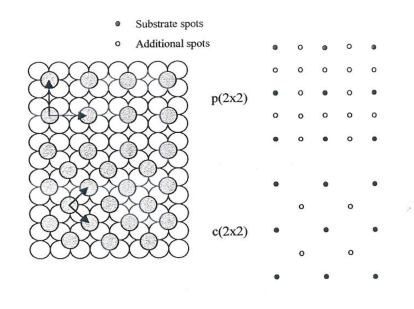
\includegraphics[scale=4]{figures/09_11.png}
	\caption{A real space model of a quarter and a half monolayer of sulphur adsorbed on Ni(100) and the respective LEED pattern.}
	\label{fig:snileed}
	\end{center}
\end{figure}

\subsubsection{Woods Notation}
Assume that the substrate is described by the basis vectors $\vec{a_1}$ and $\vec{a_2}$. The new basis vectors describing the surface structure are then $\vec{b_1}$ and  $\vec{b_2}$. In Woods notation this is described as S-Ni(100) $(\vec{b_1}/\vec{a_1}\times\vec{b_2}\vec{a_2})R\theta^{\circ}$ telling us that it is a $2\times 2$ structure of sulphur on  Ni(100) rotated $\theta$ degrees. Woods notation is quite convenient, but cannot be used to describe all LEED structures. When the angle between the new basis vectors in real space is changed with respect to the angle between the  substrate vectors the notation is no longer valid and we must use the matrix notation which is always valid.

\subsubsection{The Matrix Notation}
The substrate is in real space represented by a matrix:

\begin{equation}
{\bf A}=\begin{pmatrix}
a_{11}	& a_{12}	\\
a_{21}	& a_{22}
\end{pmatrix}
\end{equation}

Similarly the new basis set can be described by the matrix:

\begin{equation}
{\bf B}=\begin{pmatrix}
b_{11}	& b_{12}	\\
b_{21}	& b_{22}
\end{pmatrix}
\end{equation}

We can now find the matrix {\bf G} which maps {\bf A} on {\bf B}

\begin{equation}
{\bf B}={\bf GA}
\end{equation}

\noindent which is the one used in matrix notation i.e. S-Ni(100) $\left(\begin{smallmatrix} g_{11}	& g_{12}	\\ g_{21}	& g_{22 }\end{smallmatrix}\right)$, which in this specific case gives S-Ni(100) $\left(\begin{smallmatrix} 2	& 0	\\ 0	& 2 \end{smallmatrix}\right)$. Please note that the same set of equations also applies for the reciprocal set of vectors i.e.

\begin{equation}
{\bf B^*}={\bf G^*A^*}
\end{equation}

In many cases it is convenient to determine ${\bf G^*}$ from the LEED pattern and then find $\vec{b_1}$ and $\vec{b_2}$ in terms of $\vec{a_1}$ and $\vec{a_2}$ by the relation

\begin{equation}
{\bf G}=(({\bf G^*})^{\mathrm{T}})^{-1}
\end{equation}

The area of the new unit cell is conveniently found as $\det({\bf G})$.

The various types of overlayer structures can be classified by {\bf G}, but that is beyond the scope of these notes and we will refer to for example \cite{Ertl, woodruff} for details.

\subsubsection{Other Examples}
Now we have the machinery ready for investigating surface structures. If we reconsider the structure above with sulphur on Ni(100) and add another quarter of a monolayer the center positions will also be occupied. The first LEED structure is often called a p$(2\times 2)$ structure while the second is called a c$(2\times 2)$ - p for primitive $2\times 2$ and c for centred $2\times 2$. The correct notation for the latter is in Woods notation S-Ni(100)($\sqrt{2}\times \sqrt{2})R\ang{45}$ or in the matrix notation S-Ni(100) $\left(\begin{smallmatrix} 1	& 1	\\ -1	& 1 \end{smallmatrix}\right)$, since this cell is smaller than the $2\times 2$. In the above examples the adsorbate lattice automatically also included the substrate lattice. Let us now look at an example where we need to look for a coincidence cell as mentioned earlier. Consider a Ni(110) surface and the respective LEED structure when oxygen is added as shown in \autoref{fig:onileed}.

\begin{figure}[h!]
	\begin{center}
	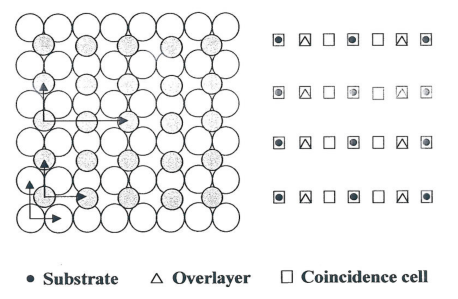
\includegraphics[scale=4]{figures/09_12.png}
	\caption{The real space model and the respective LEED patterns for the substrate, the overlayer, and the coincidence cell for oxygen on Ni(110).}
	\label{fig:onileed}
	\end{center}
\end{figure}

Let us assume that 2/3 of a monolayer oxygen has been adsorbed and that the oxygen is sitting in two non-equivalent positions. The LEED pattern from the substrate is indicated as dots. The LEED pattern from the oxygen overlayer is indicated as triangles, whereas the spots occurring from the coincidence cell is shown as open squares. Please note that the correct LEED pattern is not just the sum of the substrate and the overlayer diffraction pattern, but that the coincidence cell which describes both at the same time must be found in order to determine the correct pattern.

The LEED pattern only gives us the size and orientation of the new unit cell  formed by the substrate and the adsorbate together. It is not possible to say anything about the actual binding site or coverage of the adsorbate from the LEED pattern alone. (The adsorbate layer can be shifted in the unit cell of the substrate without any consequence for the resulting LEED pattern.) This must be determined from other experiments such as XPS and AES concerning the coverage and HREELS, STM and UPS concerning the actual binding site.

\subsection{Domains}

\begin{figure}[h!]
	\begin{center}
	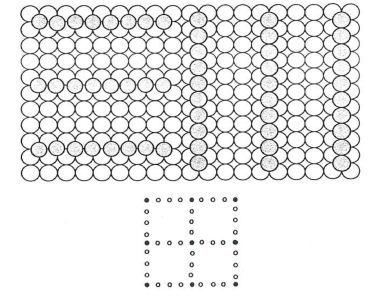
\includegraphics[scale=4]{figures/09_13.png}
	\caption{The real space model for two different domains of $4\times 1$ structure on Ni(100). The respective LEED pattern shows the result of both types of domains present on the surface.}
	\label{fig:41nileed}
	\end{center}
\end{figure}

Yet another effect may complicate the analysis of LEED patterns namely \emph{domains}. Remember that in a typical LEED experiment the electron beam probes an area of a diameter of \SIrange{0.1}{1.0}{mm} and that if we just have islands which are larger than the transfer width then we will obtain nice LEED patterns from these islands (the intensity naturally being proportional to the coverage of these islands). Due to the surface symmetry these islands may differ in orientation. Consider for example a simple $4\times 1$ structure on Ni(100) as shown in \autoref{fig:41nileed}. When this structure nucleate there will be two equal possibilities of orienting the island on a (100) surface. As we will be sampling over many islands that are randomly oriented in two-dimensions the resulting LEED pattern will simply be the sum of the LEED patterns for each type domain.

In some cases for instance if the temperature is kept low there will not be any high mobility on the surface and there will be many small domains resulting in broadening of the spots since the number of scatterers in each island are too low. This occurs if there are many small domains that are out of phase. If the different domains are in phase a sharp LEED pattern is still obtained. See \autoref{fig:22nileed} for an example.

\begin{figure}[h!]
	\begin{center}
	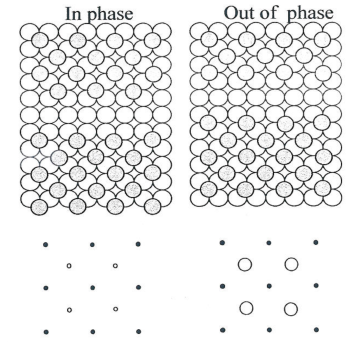
\includegraphics[scale=4]{figures/09_14.png}
	\caption{The real space model for two $2\times 2$ domains in phase and out of phase on a Ni(100) surface. Please note that in the out of phase mode the half order spots broaden if the domains are small enough.}
	\label{fig:22nileed}
	\end{center}
\end{figure}

\section{Dynamical Scattering and IV-Curves}
Strong oscillations appears in the intensity versus the  primary energy of the electrons due to the multiple scattering in the different layers. The resulting curves are called IV-curves as shown in \autoref{fig:ivni}.  The modulation are due to Bragg reflections into the crystal, but as the intensity into the bulk is exponentially damped and thus only  few layers contribute to this effect the modulation will be rather broad and the intensity will never go to zero completely.  By performing very detailed analysis of the electrons scattered in the surface and calculate the resulting beam intensity for a number of different beams as a function of energy it is possible to compare to the experimental measured IV curves.

\begin{figure}[h!]
	\begin{center}
	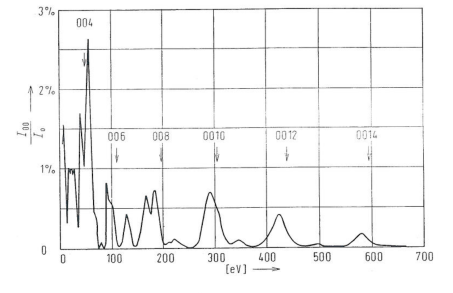
\includegraphics[scale=4]{figures/09_15.png}
	\caption{The $IV$-curve for Ni(100) at normal incidence.}
	\label{fig:ivni}
	\end{center}
\end{figure}

In this manner it is possible to obtain models which gives the best fit to the  data and obtain not only information on the two-dimensional structure in the surface but also the in depth distances between the different layers. In this manner it is for example possible to show that a clean  surface introduces an inward relaxation of the first layer towards the second while the second layer usually expands compared to the bulk lattice distances. The relaxations are typically \SIrange{-5}{10}{\percent} for the first layer and \SIrange{1}{3}{\percent} for the second layer. These relaxations are easily explained in terms of EMT. The outermost atoms are less coordinated and are therefore missing electron density. They can compensate for this and obtain the optimum electron density by shifting slightly towards the atoms below leading to the contraction. This on the other hand leads to a too high electron density for the atoms in the second layer which then expands to compensate, resulting in the so called Friedel oscillations which are exponentially damped into the material. Similarly detailed models can be constructed for adsorbate system and the distances can be extracted being the source of many accurate determinations of surface structures, see \cite{Somorjai}. Unfortunately this scheme only works for relative simple structures since the number of fitting parameter describing the IV-curves  are becoming too large for big unit cells like for instance a $\sqrt{19}\times\sqrt{19}$.

\section{Problems}
\begin{enumerate}
\item An often encountered reconstruction on metals are the missing row reconstruction of the fcc(110) surface (for example Pt(110)), where every second row of the surface are missing. Make a model of the surface in real space and its respective LEED pattern superimposed on the LEED pattern of the non-reconstructed surface. Discuss how and why this surface reconstruction appears.

\item Sulfur is adsorbed on a Ni(100) surface in a four-fold-hollow site. Draw the LEED pictures of a p($2\times 2$) and a ($2\times 1$) structure with two domains. How can you distinguish the two surfaces?

\begin{figure}[h!]
	\begin{center}
	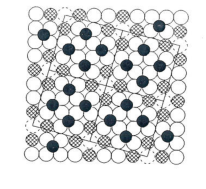
\includegraphics[scale=4]{figures/09_16.png}
	\caption{Hard sphere model of sulfur on Cu(100). Black and hatched spheres are sulfur atoms in first and second layer, respectively. Open circles and dotted circles are Cu atoms in first and second layer, respectively.}
	\label{fig:hardsphere_S_on_Cu}
	\end{center}
\end{figure}

\item Enclosed in figure \autoref{fig:hardsphere_S_on_Cu} is the hard sphere model for sulfur adsorbed on Cu(100) depicted. What is the Woods notation of the structure? What is the notation in the matrix notation? What is the coverage of sulfur and how manyu domains can be present? Draw the LEED pattern.

\item Make a few examples yourself in real space. Try for example $\sqrt3\times \sqrt3$ on a Fe(111) surface and find the resulting LEED pattern. Discuss whether the adsorbate coverage or position can be deduced for a LEED pattern.

\begin{figure}[h!]
	\begin{center}
	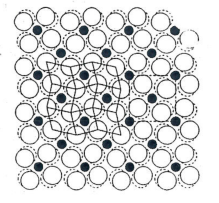
\includegraphics[scale=4]{figures/09_17.png}
	\caption{Hard sphere model of the C-NI($2\times 2$)p4g reconstruction. The black spheres are the carbon atoms while the open circles illustrates the Ni atoms displaced slightly from the original Ni(100) positions (dotted circles)}
	\label{fig:hardsphere_C_Ni}
	\end{center}
\end{figure}

\item In figure~\autoref{fig:hardsphere_C_Ni} is a hard sphere model for the clock reconstruction of carbon on Ni(100) depicted. The structure belongs to the symmetry group p4g and the resulting LEED pattern is the same as depicted in figure~\autoref{fig:culeed}. Notice that every second spot along the x and y axis is missing. Explain the reason for this peculiar behaviour.

\item In a LEED experiment we take a picture and observe a square pattern where the distance from (0,0) spit to the (1,0) spot is measured to be 4.1\,cm. Assume that the pictures is a one to one representation of the experiment. The radius of the LEED optics is 8.0\,cm and the primary energy is 72\,eV. What is the lattice distance of this crystal? If we assume there is an uncertaincy of 0.1\,cm on the measurement of the distance, what is then the resulting uncertaincy on the lattice distance determined? Discuss the energy of the electrons when being scattered at the surface.

\end{enumerate}

